\documentclass[11pt,letterpaper]{article}
\usepackage[margin=1in]{geometry}
\usepackage[T1]{fontenc}
\usepackage{lmodern,booktabs,longtable,array,graphicx,amsmath,natbib,setspace}
\usepackage[font=small,labelfont=bf]{caption}
\usepackage[hidelinks]{hyperref}
\usepackage{microtype}
\setstretch{1.12}
\widowpenalty=10000
\clubpenalty=10000
\setlength{\emergencystretch}{2em}
\graphicspath{{../figs/}}
\newcommand{\RareOne}{6.2}
\newcommand{\CombinedOne}{24.6}
\newcommand{\InsincereOne}{8.8}
\newcommand{\RareTwo}{30.0}
\newcommand{\CombinedTwo}{37.9}
\newcommand{\InsincereTwo}{14.4}
\newcommand{\RareThree}{21.0}
\newcommand{\CombinedThree}{27.6}
\newcommand{\InsincereThree}{14.3}
\newcommand{\AllJobs}{-0.096}
\newcommand{\AllPrices}{-0.060}
\newcommand{\CleanJobs}{-0.125}
\newcommand{\CleanPrices}{-0.091}
\newcommand{\FlaggedJobs}{-0.049}
\newcommand{\FlaggedPrices}{-0.013}
\newcommand{\IpOne}{20.3}
\newcommand{\IpTwo}{12.1}
\newcommand{\IpThree}{9.8}
\newcommand{\ReductionJobs}{23.0}
\newcommand{\ReductionLowJobs}{4.2}
\newcommand{\ReductionHighJobs}{38.7}
\newcommand{\ReductionPrices}{33.9}
\newcommand{\ReductionLowPrices}{9.2}
\newcommand{\ReductionHighPrices}{56.9}

\newcommand{\tabnote}[1]{\par\smallskip{\footnotesize #1\par}}
\title{The Micro-Task Market for Lemons:\\Data Quality on Amazon's Mechanical Turk\\[0.5em]\large Updated replication and measurement assessment}
\author{Douglas J. Ahler \and Carolyn E. Roush \and Gaurav Sood}
\date{Replication edition: October 9, 2026}
\begin{document}
\maketitle
\begin{abstract}
\noindent Response-quality screens flag a substantial share of records in three surveys collected on Amazon's Mechanical Turk. IP flags decrease from \IpOne\% in August 2018 to \IpThree\% in July 2020, while endorsement of multiple uncommon traits rises from \RareOne\% to \RareThree\%. Combining the screens flags \CombinedOne\%, \CombinedTwo\%, and \CombinedThree\% in the August 2018, June 2020, and July 2020 surveys. In a randomized economic-evaluation experiment, an out-party rather than an in-party cue lowers unemployment evaluations by \AllJobs{} on a zero-to-one scale in the full sample and by \CleanJobs{} among unflagged records. The full-sample contrast is \ReductionJobs\% smaller (95\% paired IP-cluster bootstrap interval: \ReductionLowJobs\% to \ReductionHighJobs\%). Screening changes the estimated contrasts, but does not identify the causal effect of dishonesty: IP metadata, reported uncommon traits, and date conventions are imperfect measures of response quality. The replication also corrects duplicate-IP coding in historical platform comparisons. These findings support reporting how recruitment and screening choices affect sample composition and inference, with the evidence confined to the archived surveys.
\end{abstract}
\noindent\small This is a revised replication manuscript, not the version of record or a journal correction. The published article is \emph{Political Science Research and Methods}, DOI \href{https://doi.org/10.1017/psrm.2021.57}{10.1017/psrm.2021.57}. Its historical text and results remain in the original materials. The results below describe the archived surveys, not the current MTurk population.\normalsize

\section{The question and the evidence}

Online labor markets lowered the cost of recruiting experimental participants and broadened recruitment beyond university subject pools \citep{sears_1986,berinsky_2012,paolacci_2010}. A low recruitment cost does not establish that respondents read questions, satisfy eligibility requirements, or report their experiences accurately. Nor does a response-quality screen by itself establish that a flagged participant is dishonest. The empirical question is how often the available screens flag a record and how the results change when those records are excluded.

The original study fielded an August 2018 survey and two additional surveys in June and July 2020. These surveys combined IP metadata, response times, questions about uncommon traits and behaviors, self-reported sincerity, and randomized experiments. The reconstructed analysis retains those design comparisons and distinguishes the archived definitions from verified coding repairs.

The distinction between a screen and a validated outcome matters throughout. A foreign IP location is not an observation of citizenship. Multiple submissions from an IP can come from a shared household or institution. Endorsing two unusual experiences is not proof of fabrication. These observations still matter to research design, but their meaning must remain narrower than the labels ``bad actor'' or ``troll'' imply.

\section{Incentives and what the design identifies}

A micro-task market connects requesters who pay for tasks with workers who complete them. Ratings can encourage effort when requesters can verify quality. Survey opinions and personal experiences are harder to verify than a classification task with a known answer. A requester may approve questionable work because checking it costs time, because the response could be sincere, or because an incorrect rejection would treat the worker unfairly. The resulting approval rate is an imperfect measure of survey response quality \citep{akerlof1978market,peer_2014}.

A managed panel can accumulate information across repeated interactions with its participants. That difference motivates comparison with MTurk, but it is not experimentally manipulated here. The studies differ in recruitment, calendar time, questionnaire, pay, and eligibility restrictions. Their comparisons describe the samples obtained under those conditions. They do not isolate the causal effect of a platform, an approval threshold, or changes in Amazon's policies. Similarly, reported task experience is associated with measured response patterns; it was not randomly assigned.

Several mechanisms could produce a flagged record: deliberate misrepresentation, inattention, misunderstanding, a valid uncommon experience, a shared network, or an imperfect location service. The archive does not supply verified labels that separate these mechanisms.

\section{Surveys, measures, and denominators}

% Design literals below are from the original manuscript, section 3; they are not estimated results.
Study 1 was fielded on August 17, 2018, advertised as a ten-minute survey, and paid \$0.60 per completed task. Study 2 was fielded in June 2020, advertised as a fifteen-minute survey, and paid \$0.75. Study 3 was fielded in July 2020, advertised as a five-minute survey, and paid \$0.35. Studies 1 and 3 required a task approval rate of at least 95\%; Study 2 did not. Each sought participants located in the United States. Table~\ref{tab:ip} reports the archived record counts; availability varies across survey items and models. In Study 1 the row unit is a paid assignment. The archive includes one observed survey response linked to two paid assignments, as well as assignments without linked survey data. The baseline retains that archived unit; a separate unique-survey sensitivity removes the repeated response and recalculates IP duplication. Neither unit identifies distinct people.

Qualtrics recorded IP addresses. The original project used Know Your IP to obtain location and blacklist information from external services \citep{kyip}. This edition uses the deposited metadata. IP addresses and blacklist status change, so querying a current service would measure something different from the original survey conditions. Public record identifiers permit counting repeated IPs without publishing addresses.

The IP screen marks records with missing addresses, a positive blacklist indicator, a repeated recorded address, or a location outside the United States. Repeated-address percentages count \emph{responses} attached to an address that appears more than once. The supplementary multiplicity table instead counts distinct observed addresses and reports how many responses those addresses contribute. Missing addresses are not one shared network. Missing blacklist information is uncertainty about that screen, not affirmative evidence that an address was absent from every blacklist.

The rare-trait screen counts affirmative answers about an artificial limb or prosthetic, vision impairment, hearing impairment, gang membership, immediate-family gang membership, and an unusual amount of sleep. The original threshold was two affirmative answers. The sleep item asks average hours per night and flags the categories ``4 or less and ``More than 10. The adjacent ``4--6 category overlaps at the boundary, so the recorded category is preserved. These are reported experiences; the screen is not a diagnosis or a validated measure of insincerity. In particular, questions about \emph{any} vision or hearing impairment cannot be compared directly with population rates of blindness or deafness, and age-restricted population estimates do not automatically match this convenience sample.

The 2020 surveys also asked participants to enter the date. Index 1 combines the IP and rare-trait screens. Index 2 additionally flags the day/month/year convention, and index 3 additionally flags entries that are not dates. These are increasingly inclusive operational definitions, not statistical lower and upper bounds on the number of dishonest or foreign participants. A date convention may reflect upbringing or habit among US residents. The data do not measure its sensitivity or specificity for location.

The original project reported that respondents passed its reCAPTCHA check. Passing an automated challenge does not establish attentive reading of the questionnaire or exclude every form of automation. Where pre-entry failures were not deposited, the replication cannot estimate the check's failure rate among all attempted entrants.

\section{Response patterns across the three surveys}

\begin{table}[htbp]\centering
\caption{Responses flagged by IP metadata}\label{tab:ip}
\begin{tabular}{lrrrrrr}
\toprule
Study & N & Missing & Blacklisted & Repeated & Foreign & Any \\
\midrule
August 2018 & 2000 & 0.5 & 16.1 & 5.3 & 6.0 & 20.3 \\
June 2020 & 1505 & 0.0 & 6.7 & 5.4 & 1.1 & 12.1 \\
July 2020 & 409 & 0.0 & 5.9 & 3.2 & 0.7 & 9.8 \\
\bottomrule
\end{tabular}

\tabnote{Percentages of survey records. Categories overlap. A duplicate is a record with an observed IP identifier occurring more than once in its survey. Study 1 rows are paid assignments, including one twice-linked observed response. These metadata identify screening conditions, not verified deception.}
\end{table}

The IP and rare-trait screens capture different aspects of the data. The combined first index flags \CombinedOne\% in August 2018, \CombinedTwo\% in June 2020, and \CombinedThree\% in July 2020. The rare-trait screen alone flags \RareOne\%, \RareTwo\%, and \RareThree\%, respectively. Table~\ref{tab:ip} compares the IP components, while Figure~\ref{fig:rare} separates the rare-trait items. Reading the screens together preserves the original paper's central descriptive comparison: a reduction in IP flags can coexist with an increase in rare-trait endorsements. The combined indices in Table~\ref{tab:screen} report their overlap rather than adding percentages that may count the same record twice.

\begin{figure}[htbp]\centering
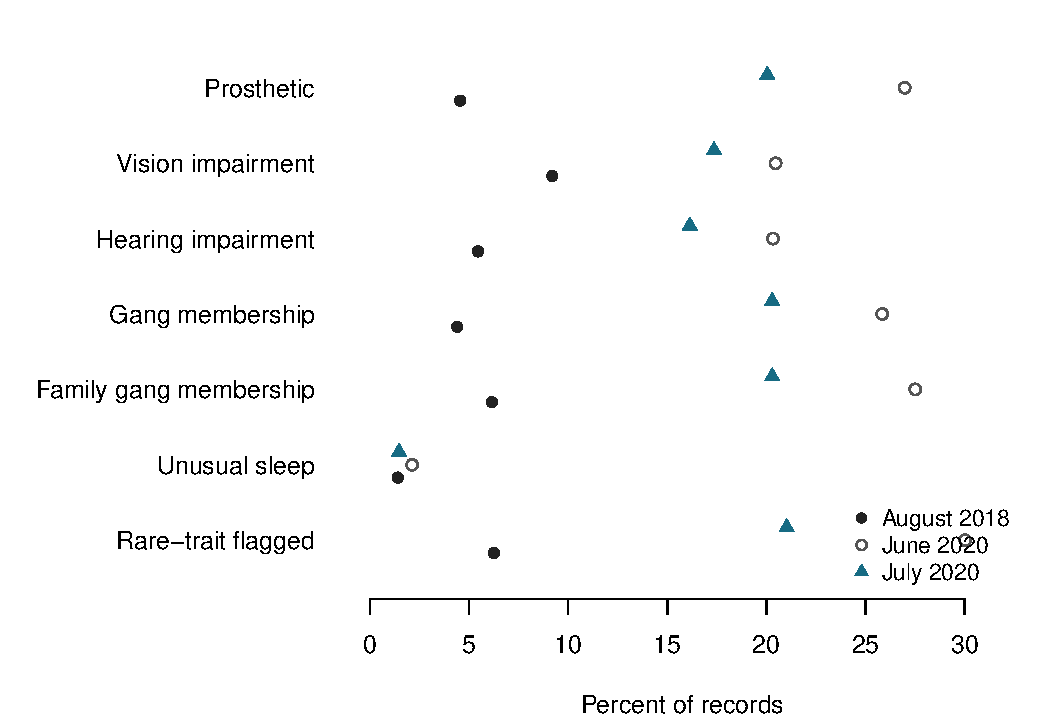
\includegraphics[width=\linewidth]{rare_traits.pdf}
\caption{Reported uncommon traits and behaviors across surveys. Points show affirmative percentages under the archived binary recodes, which treat missing rare-trait responses as negative. The final screen combines the archived rare-trait items. These are descriptive sample proportions, not population prevalence estimates.}\label{fig:rare}
\end{figure}

\begin{table}[htbp]\centering
\caption{Combined screens and self-reported insincerity}\label{tab:screen}
\begin{tabular}{lrrr}
\toprule
Measure & August 2018 & June 2020 & July 2020 \\
\midrule
Rare-trait flagged & 6.2 & 30.0 & 21.0 \\
Insincerity & 8.8 & 14.4 & 14.3 \\
Insincerity: some or more & 8.8 & 33.3 & 28.5 \\
Index 1 & 24.6 & 37.9 & 27.6 \\
Index 2 & -- & 44.6 & 35.2 \\
Index 3 & -- & 46.2 & 35.2 \\
Day-first date & -- & 20.0 & 16.4 \\
Non-date & -- & 4.9 & 4.2 \\
\bottomrule
\end{tabular}

\tabnote{Percentages use observed values of the named measure; unavailable items are shown as --. Historical insincerity counts some/most/always in 2018 and most/always in 2020; the next row uses some/most/always throughout. Indices 2 and 3 add date-format and non-date flags to index 1. The indices are alternative definitions, not identified bounds on response quality.}
\end{table}

The self-report of humorous or insincere responding provides a separate comparison with the rare-trait screen. The original main analysis used ``some of the time or more in 2018 but ``most of the time or more in 2020. Table~\ref{tab:screen} labels those historical thresholds and additionally reports a common ``some of the time threshold across all three surveys. Changes in the historical row must not be interpreted as changes in an identically defined measure. Their association is informative, but the measures do not validate one another against observed truth. Both can be affected by misunderstanding or response style. Supplementary tables show the cross-tabulations, their denominators, and tests of association.

\subsection{Experience and completion times}

Respondents in the 2020 surveys reported a category for the number of tasks they had completed. Table~\ref{tab:hits} reports screen prevalence, self-reported insincerity, and average duration within those categories. The pattern can inform recruitment choices, but it cannot establish what would happen if an otherwise identical requester imposed a new threshold. Experienced respondents may read more efficiently, differ in other characteristics, or recognize familiar designs. Those explanations are not separated by these data.

\begin{table}[htbp]\centering
\caption{Screening and duration by reported task experience}\label{tab:hits}
\textbf{June 2020}\par\smallskip
\begin{tabular}{lrrrr}
\toprule
Measure & Under 100 & 100--500 & 500--1,000 & Over 1,000 \\
\midrule
Sample share & 21.8 & 29.0 & 12.8 & 36.5 \\
Index 1 & 56.0 & 51.5 & 45.3 & 14.1 \\
Index 2 & 68.8 & 60.2 & 51.6 & 15.3 \\
Index 3 & 70.0 & 60.9 & 53.6 & 17.5 \\
Insincerity & 14.7 & 23.0 & 16.7 & 6.6 \\
Duration (seconds) & 678.3 & 608.5 & 586.2 & 495.9 \\
\bottomrule
\end{tabular}
\par\medskip
\textbf{July 2020}\par\smallskip
\begin{tabular}{lrrrr}
\toprule
Measure & Under 100 & 100--500 & 500--1,000 & Over 1,000 \\
\midrule
Sample share & 20.7 & 26.8 & 9.4 & 43.1 \\
Index 1 & 50.0 & 40.4 & 31.6 & 6.9 \\
Index 2 & 63.1 & 51.4 & 34.2 & 10.9 \\
Index 3 & 63.1 & 51.4 & 34.2 & 10.9 \\
Insincerity & 14.3 & 24.8 & 34.2 & 3.4 \\
Duration (seconds) & 544.9 & 490.8 & 452.2 & 280.5 \\
\bottomrule
\end{tabular}
\par\medskip
\tabnote{Entries are percentages except mean duration in seconds. Task counts are self-reported categories. Item denominators are recorded in the accompanying CSV.}
\end{table}


Timing is also an imperfect proxy for quality. A short duration can reflect speed or familiarity; a long duration can include a break. Supplementary tables report quartiles, median duration, and the original study's timing screens. Missing durations remain missing when classifying slow and fast respondents. Tests that fail to reject a treatment interaction do not show that the groups have equivalent responsiveness: the interval determines which differences remain compatible with the data.

\section{Comparisons with other platforms}

The publication compared these surveys with earlier MTurk surveys and with SSI/Dynata and Lucid samples \citep{ahler_broockman,coppock2019validating,graham_dk_2019,graham_corona_2020,thompson_busby_2020}. The audit found two coding problems in these comparisons: some historical duplicate flags were computed across separate surveys, and one combined Lucid flag used a duplicate vector from the wrong dataset. Table~\ref{tab:platform} gives the original and corrected percentages. These repairs change particular platform comparisons and therefore the numerical basis of blanket claims about their relative quality. Some source datasets cannot be redistributed in this public package. Table~\ref{tab:platform} therefore identifies deposited aggregates as historical comparisons and labels the three studies that can be recomputed. Availability of local private data does not make those data part of the public replication.

{\small
\begin{longtable}{>{\raggedright\arraybackslash}p{0.254157303370787\linewidth}>{\raggedright\arraybackslash}p{0.078876404494382\linewidth}>{\raggedright\arraybackslash}p{0.140224719101124\linewidth}>{\raggedright\arraybackslash}p{0.0964044943820225\linewidth}>{\raggedright\arraybackslash}p{0.105168539325843\linewidth}>{\raggedright\arraybackslash}p{0.105168539325843\linewidth}}
\caption{IP-flagged responses across surveys (percent)\label{tab:platform}}\\
\toprule
Survey & Year & Platform & N & Flagged & Unknown \\
\midrule\endfirsthead
\toprule
Survey & Year & Platform & N & Flagged & Unknown \\
\midrule\endhead
\bottomrule\endfoot
Busby & 2019 & Lucid & 2531 & 2.84 & 0 \\
Graham August & 2019 & Lucid & 8555 & 4.18 & 0 \\
Graham June & 2019 & Lucid & 7068 & 2.02 & 0 \\
Thompson and Busby & 2019 & Lucid & 1798 & 1.61 & 0 \\
Graham & 2020 & Lucid & 4233 & 1.89 & 1 \\
Ahler and Broockman & 2015 & MTurk & 2045 & 12.42 & 0 \\
Ahler and Goggin & 2015 & MTurk & 898 & 5.68 & 0 \\
August survey & 2018 & MTurk & 2000 & 20.30 & 0 \\
July survey & 2020 & MTurk & 409 & 9.78 & 0 \\
June survey & 2020 & MTurk & 1505 & 12.09 & 0 \\
Berkeley IGS Poll & 2015 & SSI/Dynata & 2295 & 4.14 & 46 \\
\end{longtable}}
\noindent\small Comparison-survey counts are supplied as aggregate inputs. Percentages use all records; Unknown counts unresolved flags. Repeated IPs are counted within each survey.\normalsize


The comparison concerns IP flags, not every dimension of data quality. A panel with fewer IP flags may still contain inattentive participants. Blacklist metadata retrieved after a survey can change with address reassignment; questionnaire and recruitment differences can also change the composition of a sample. Consequently, these comparisons do not identify the relative causal performance of the platforms or establish current procurement advice.

The paper also compared cost per response-minute after removing IP-flagged records. That quantity is payment plus the assumed platform charge, divided by the fraction retained and the assumed survey length. It is a cost per \emph{unflagged} response-minute, not a validated cost per truthful response. Advertised and observed durations answer different questions, and nominal charges in the original study are historical inputs. Modern prices must not be inferred from this calculation.

\begin{table}[htbp]\centering
\caption{Historical cost per IP-unflagged response-minute}
\resizebox{\linewidth}{!}{
\begin{tabular}{lrrrrr}
\toprule
Study & Dollars & Multiplier & Minutes & Flagged & Cents \\
\midrule
June 2020 & 0.75 & 1.3 & 15 & 12.1 & 7.39 \\
July 2020 & 0.35 & 1.3 & 5 & 9.8 & 10.09 \\
Lucid illustrative & 1.00 & 1.0 & 10 & 2.0 & 10.20 \\
Lucid targeted illustrative & 2.00 & 1.0 & 10 & 1.6 & 20.33 \\
\bottomrule
\end{tabular}
}
\par\smallskip
\noindent\small Dollars is payment per response. Cents is the cost per retained response-minute, including the historical fee multiplier. Lucid rows preserve illustrative published price, duration, and rounded IP-rate assumptions; they are not updated vendor quotations.\normalsize\end{table}


\section{Experimental treatment effects and screening}

The June 2020 experiment asked partisans to evaluate small decreases in unemployment and inflation. A randomly assigned cue attributed the period either to President Obama or to Republican control of Congress. The analysis codes the cue relative to the respondent's party, including partisan leaners, and compares an out-party cue with an in-party cue. Responses run from worse to better on a scale from zero to one. The questionnaire wording appears in the appendix.

For each outcome, the subgroup model is
\begin{equation}
Y_i=\beta_0+\beta_1 T_i+\beta_2 F_i+\beta_3 T_iF_i+\varepsilon_i,
\end{equation}
where $T_i$ indicates the out-party cue and $F_i$ is the specified flag. Figure~\ref{fig:effects} reports subgroup contrasts on the observed outcome scale, including their uncertainty. Supplementary tables give the corresponding model results. A negative effect means less favorable assessment under the out-party cue.

\begin{figure}[htbp]\centering
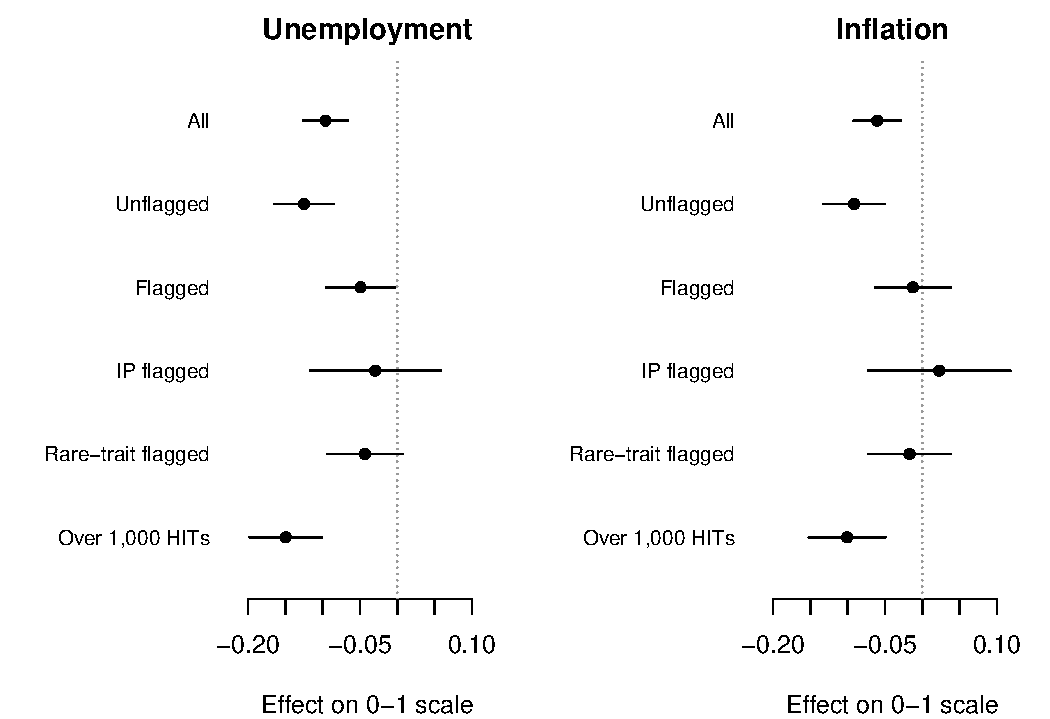
\includegraphics[width=\linewidth]{experiment_effects.pdf}
\caption{Out-party versus in-party cues in the June 2020 experiment. Points are estimated differences on the zero-to-one economic evaluation scale; lines show 95\% confidence intervals from the fitted models. Samples are item-complete partisan respondents within each reported subgroup. Different subgroup point estimates are not themselves a test of the between-group difference.}\label{fig:effects}
\end{figure}

The full-sample contrasts are \AllJobs{} for unemployment and \AllPrices{} for inflation. The corresponding unflagged contrasts are \CleanJobs{} and \CleanPrices{}; the flagged contrasts are \FlaggedJobs{} and \FlaggedPrices{}. The appendix shows the arm-specific outcome means and endpoint shares, so the treatment differences can be assessed against their baseline response levels. Conventional, heteroskedasticity-robust, and IP-clustered estimates are retained in the generated results; the appendix gives the clustered intervals.

Randomization supports comparisons between assigned cues within the experimental sample. Flagged and unflagged respondents were not randomly assigned to their screening status. Interpreting a subgroup difference as the effect of dishonesty requires assumptions about what the flag measures and whether its measurement can depend on treatment. The unflagged subgroup is a different analysis population, not an observed error-free counterfactual for the full sample. The original model-based comparison remains useful as a screening sensitivity analysis.

\subsection{What attenuation means here}

Additive mean-zero measurement error in an outcome increases uncertainty without necessarily attenuating a randomized treatment contrast. Attenuation instead follows from a particular response-replacement model. Let $Y_i^*$ be a meaningful response, let $R_i$ identify a replacement response, and write
\begin{equation}
Y_i=(1-R_i)Y_i^*+R_i Z_i.
\end{equation}
If replacement occurs with probability $q$ independently of treatment and the relevant potential outcomes, and $Z_i$ has the same expectation in each treatment arm, then
\begin{equation}
E[Y_i\mid T_i=1]-E[Y_i\mid T_i=0]=(1-q)\tau,
\end{equation}
where $\tau$ is the meaningful-response treatment contrast. Systematic or treatment-dependent replacement need not move the estimate toward zero. The screen comparisons do not identify $q$ or establish this mechanism.

For the empirical comparison, define the retention ratio as the full-sample contrast divided by the unflagged-sample contrast. Subtracting that ratio from one gives a relative reduction, expressed as a percentage after multiplication by one hundred. Subtracting the contrasts themselves gives a difference on the outcome scale; multiplying that difference by one hundred yields percentage points only when the outcome is a probability or proportion. Ratios are unstable when their denominator is near zero. Because full and unflagged estimates share observations, their uncertainties are dependent. A pooled ratio must state its weights and propagate that dependence.

{\small
\begin{longtable}{>{\raggedright\arraybackslash}p{0.108837209302326\linewidth}>{\raggedright\arraybackslash}p{0.181395348837209\linewidth}>{\raggedright\arraybackslash}p{0.0634883720930233\linewidth}>{\raggedright\arraybackslash}p{0.108837209302326\linewidth}>{\raggedright\arraybackslash}p{0.0634883720930233\linewidth}>{\raggedright\arraybackslash}p{0.108837209302326\linewidth}>{\raggedright\arraybackslash}p{0.0725581395348837\linewidth}>{\raggedright\arraybackslash}p{0.0725581395348837\linewidth}}
\caption{Full-sample and unflagged contrasts: descriptive retention ratios}\\
\toprule
Study & Contrast & Full & Unflagged & Ratio & Reduction & Lower & Upper \\
\midrule\endfirsthead
\toprule
Study & Contrast & Full & Unflagged & Ratio & Reduction & Lower & Upper \\
\midrule\endhead
\bottomrule\endfoot
August 2018 & Black x -1 & 0.117 & 0.140 & 0.839 & 16.1 & -0.1 & 31.1 \\
August 2018 & Black x 1 & 0.082 & 0.097 & 0.847 & 15.3 & -0.6 & 30.6 \\
August 2018 & Same-sex spouse x -1 & 0.165 & 0.191 & 0.868 & 13.2 & 1.5 & 24.3 \\
August 2018 & Same-sex spouse x 1 & 0.115 & 0.132 & 0.876 & 12.4 & 0.4 & 23.6 \\
August 2018 & Evangelical x -1 & 0.044 & 0.059 & 0.750 & 25.0 & -49.7 & 101.3 \\
August 2018 & Evangelical x 1 & 0.031 & 0.042 & 0.752 & 24.8 & -50.3 & 101.3 \\
August 2018 & Secular x -1 & 0.067 & 0.066 & 1.026 & -2.6 & -137.5 & 48.2 \\
August 2018 & Secular x 1 & 0.046 & 0.045 & 1.031 & -3.1 & -134.8 & 47.8 \\
August 2018 & Liberal activity x -1 & 0.080 & 0.094 & 0.852 & 14.8 & -28.8 & 42.6 \\
August 2018 & Liberal activity x 1 & 0.055 & 0.064 & 0.859 & 14.1 & -27.8 & 41.9 \\
August 2018 & Conservative activity x -1 & 0.088 & 0.083 & 1.059 & -5.9 & -89.5 & 23.1 \\
August 2018 & Conservative activity x 1 & 0.063 & 0.059 & 1.069 & -6.9 & -92.0 & 22.9 \\
June 2020 & Unemployment & -0.096 & -0.125 & 0.770 & 23.0 & 4.2 & 38.7 \\
June 2020 & Inflation & -0.060 & -0.091 & 0.661 & 33.9 & 9.2 & 56.9 \\
\end{longtable}}
\noindent\small Reduction is 100 times one minus the retention ratio. It is a descriptive relative change, not the causal effect of dishonesty. James contrasts are sign-aligned to the unflagged estimate; those signs cancel in the ratios. Lower and Upper are 95 percent percentile intervals for the relative reduction from a paired IP-cluster bootstrap; full and unflagged estimates are refitted in each draw. Respondent-bootstrap results are also supplied in CSV.\normalsize


\section{Implications for survey research}

The data support examining several response-quality indicators and showing how conclusions change under prespecified screens. They do not support equating a disability, a date convention, or a shared IP address with misconduct. Researchers should distinguish eligibility checks, attentive reading, response consistency, and intentional fabrication, because each asks a different question and may require different evidence.

The original recommendations included checking location and repeated submissions, including response-quality items, allowing time to inspect data, considering task experience, and comparing costs across recruitment sources. Those remain design choices to evaluate against their measurement error and effects on sample composition. Participants should know the task and compensation conditions before consenting. Quality bonuses and alternative rating systems are hypotheses about incentives, not interventions tested in these surveys.

IP collection also depends on consent, institutional requirements, and applicable law. Where IP collection is unavailable, other screens can provide information, but neither date conventions nor rare-trait questions are validated substitutes for a participant's location. Any exclusion strategy should report missingness, the records removed, and sensitivity of the substantive findings. The scope of this replication is the archived evidence; the current quality and prices of online recruitment platforms require new data.

\clearpage
\bibliographystyle{plainnat}
\bibliography{references}
\clearpage
\appendix
\section{Reproduction, corrections, and coverage}

The archived package combines R summaries, Stata survey analysis, and manually assembled exhibits. The rebuilt pipeline separates data coding, estimation, and presentation. Counts and membership are checked exactly where historical evidence permits; fitted estimates are checked with explicit tolerances. Original-code execution and an R reconstruction are distinct forms of evidence and are labeled in the accompanying comparison outputs. Model intervals concern individual contrasts and do not adjust for simultaneous examination of many outcomes. The descriptive sample rates do not acquire population representativeness from a large number of observations.

{\small
\begin{longtable}{>{\raggedright\arraybackslash}p{0.141818181818182\linewidth}>{\raggedright\arraybackslash}p{0.212727272727273\linewidth}>{\raggedright\arraybackslash}p{0.106363636363636\linewidth}>{\raggedright\arraybackslash}p{0.106363636363636\linewidth}>{\raggedright\arraybackslash}p{0.106363636363636\linewidth}>{\raggedright\arraybackslash}p{0.106363636363636\linewidth}}
\caption{Changed survey proportions after missing-value repairs}\\
\toprule
Study & Measure & Original & Corrected & OriginalN & CorrectedN \\
\midrule\endfirsthead
\toprule
Study & Measure & Original & Corrected & OriginalN & CorrectedN \\
\midrule\endhead
\bottomrule\endfoot
August 2018 & Fast timing screen & 2.050 & 2.059 & 2000 & 1991 \\
August 2018 & Slow timing screen & 11.650 & 11.251 & 2000 & 1991 \\
July 2020 & Insincerity (historical) & 14.181 & 14.251 & 409 & 407 \\
\end{longtable}}


The following tables cover the supporting analyses: distributions of observed IP multiplicity and recorded geography; associations between screens; timing distributions and models; subgroup experiments; and ordered-logit models for the James experiment. Country and city labels describe the deposited geolocation service's output. They do not establish residence. The original manual interpretation of the timing of repeated submissions is not reproduced merely by counting duplicates: separating coordinated individuals from one person using several devices requires information these records do not identify.

{\small
\begin{longtable}{lrrr}
\caption{Observed IP multiplicity: addresses and response records}\\
\toprule
study & multiplicity & n addresses & n responses \\
\midrule\endfirsthead
\toprule
study & multiplicity & n addresses & n responses \\
\midrule\endhead
\bottomrule\endfoot
August 2018 & 1 & 1885 & 1885 \\
August 2018 & 2 & 20 & 40 \\
August 2018 & 3 & 13 & 39 \\
August 2018 & 4 & 4 & 16 \\
August 2018 & 5 & 1 & 5 \\
August 2018 & 6 & 1 & 6 \\
June 2020 & 1 & 1424 & 1424 \\
June 2020 & 2 & 33 & 66 \\
June 2020 & 3 & 3 & 9 \\
June 2020 & 6 & 1 & 6 \\
July 2020 & 1 & 396 & 396 \\
July 2020 & 2 & 5 & 10 \\
July 2020 & 3 & 1 & 3 \\
\end{longtable}}
{\small
\begin{longtable}{lrr}
\caption{Response records by recorded country}\\
\toprule
study & location & n \\
\midrule\endfirsthead
\toprule
study & location & n \\
\midrule\endhead
\bottomrule\endfoot
August 2018 & Canada & 6 \\
August 2018 & India & 17 \\
August 2018 & Other & 54 \\
August 2018 & United States & 1870 \\
August 2018 & Venezuela & 42 \\
June 2020 & India & 12 \\
June 2020 & Other & 5 \\
June 2020 & United States & 1488 \\
July 2020 & Other & 3 \\
July 2020 & United States & 406 \\
\end{longtable}}
{\small
\begin{longtable}{lrr}
\caption{Response records by recorded city}\\
\toprule
study & location & n \\
\midrule\endfirsthead
\toprule
study & location & n \\
\midrule\endhead
\bottomrule\endfoot
August 2018 & Buffalo & 77 \\
August 2018 & Kansas City & 28 \\
August 2018 & Los Angeles & 44 \\
August 2018 & Maracaibo & 31 \\
August 2018 & New York & 72 \\
August 2018 & Other & 1601 \\
June 2020 & Chicago & 40 \\
June 2020 & Las Vegas & 35 \\
June 2020 & Los Angeles & 52 \\
June 2020 & New York & 31 \\
June 2020 & Other & 1224 \\
July 2020 & Other & 384 \\
\end{longtable}}
{\small
\begin{longtable}{>{\raggedright\arraybackslash}p{0.159354838709677\linewidth}>{\raggedright\arraybackslash}p{0.0754838709677419\linewidth}>{\raggedright\arraybackslash}p{0.109032258064516\linewidth}>{\raggedright\arraybackslash}p{0.109032258064516\linewidth}>{\raggedright\arraybackslash}p{0.109032258064516\linewidth}>{\raggedright\arraybackslash}p{0.109032258064516\linewidth}>{\raggedright\arraybackslash}p{0.109032258064516\linewidth}}
\caption{Sensitivity of screen counts to missing rare-trait items}\\
\toprule
Study & N & Missing & RareMin & RareMax & IndexMin & IndexMax \\
\midrule\endfirsthead
\toprule
Study & N & Missing & RareMin & RareMax & IndexMin & IndexMax \\
\midrule\endhead
\bottomrule\endfoot
August 2018 & 2000 & 9 & 125 & 134 & 493 & 493 \\
June 2020 & 1505 & 4 & 452 & 455 & 571 & 574 \\
July 2020 & 409 & 2 & 86 & 88 & 113 & 113 \\
\end{longtable}}
\noindent\small Minimum sets missing rare-trait items to negative; maximum sets them to affirmative. These bound the screen under missing answers, not the number of dishonest participants.\normalsize

\begin{figure}[htbp]\centering
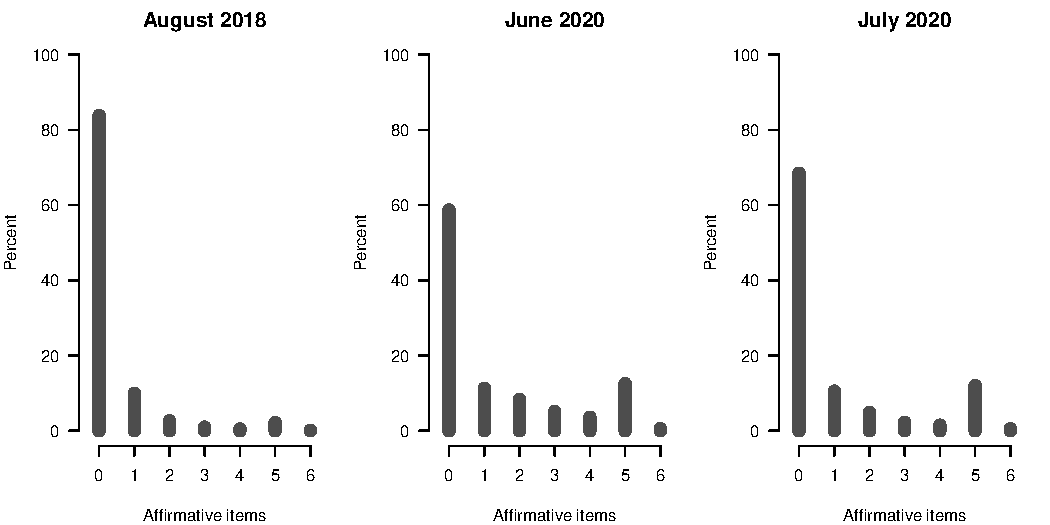
\includegraphics[width=\linewidth]{rare_counts.pdf}
\caption{Distribution of the number of affirmative rare-trait items. Each panel uses the archived item recodes and the same percentage scale.}
\end{figure}
\begin{figure}[htbp]\centering
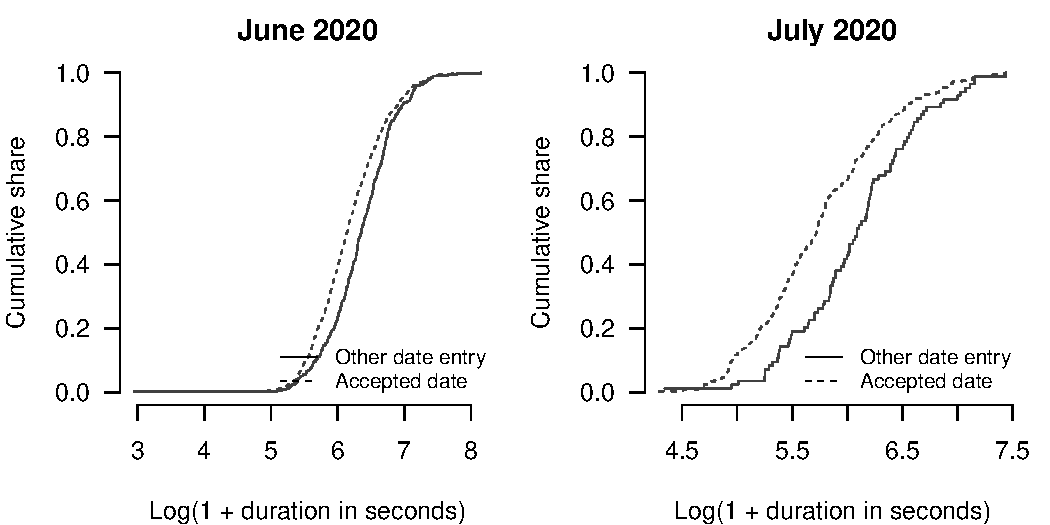
\includegraphics[width=\linewidth]{date_timing.pdf}
\caption{Duration distributions by date convention in the two 2020 surveys. Empirical cumulative distributions compare accepted date entries with other entries, including non-dates, and retain long completion times on a logarithmic time axis. Date convention does not establish location or citizenship.}
\end{figure}
{\small
\begin{longtable}{lrrrrrr}
\caption{Associations with the rare-trait screen}\\
\toprule
Study & Measure & Screen & N & Percent & ChiSq & p \\
\midrule\endfirsthead
\toprule
Study & Measure & Screen & N & Percent & ChiSq & p \\
\midrule\endhead
\bottomrule\endfoot
August 2018 & Insincerity & Not rare-trait flagged & 1865 & 6.6 & 179.0 & <0.001 \\
August 2018 & Insincerity & Rare-trait flagged & 125 & 41.6 & 179.0 & <0.001 \\
August 2018 & IP flagged & Not rare-trait flagged & 1875 & 19.6 & 8.4 & 0.004 \\
August 2018 & IP flagged & Rare-trait flagged & 125 & 30.4 & 8.4 & 0.004 \\
June 2020 & Insincerity & Not rare-trait flagged & 1051 & 10.2 & 49.9 & <0.001 \\
June 2020 & Insincerity & Rare-trait flagged & 452 & 24.1 & 49.9 & <0.001 \\
June 2020 & IP flagged & Not rare-trait flagged & 1053 & 11.3 & 2.1 & 0.150 \\
June 2020 & IP flagged & Rare-trait flagged & 452 & 13.9 & 2.1 & 0.150 \\
July 2020 & Insincerity & Not rare-trait flagged & 321 & 12.1 & 5.5 & 0.019 \\
July 2020 & Insincerity & Rare-trait flagged & 86 & 22.1 & 5.5 & 0.019 \\
July 2020 & IP flagged & Not rare-trait flagged & 323 & 8.4 & 3.5 & 0.061 \\
July 2020 & IP flagged & Rare-trait flagged & 86 & 15.1 & 3.5 & 0.061 \\
\end{longtable}}
{\small
\begin{longtable}{lrrrrrrr}
\caption{Survey duration in seconds by screening group}\\
\toprule
Study & Group & N & Mean & SD & Q1 & Median & Q3 \\
\midrule\endfirsthead
\toprule
Study & Group & N & Mean & SD & Q1 & Median & Q3 \\
\midrule\endhead
\bottomrule\endfoot
August 2018 & All & 1991 & 679.5 & 410.4 & 426.0 & 573.0 & 785.0 \\
August 2018 & Flagged & 484 & 805.1 & 497.7 & 467.5 & 659.5 & 1017.0 \\
August 2018 & Unflagged & 1507 & 639.2 & 369.4 & 420.0 & 554.0 & 727.0 \\
June 2020 & All & 1505 & 579.1 & 345.4 & 349.0 & 488.0 & 721.0 \\
June 2020 & Flagged & 571 & 615.9 & 339.4 & 393.0 & 543.0 & 767.0 \\
June 2020 & Unflagged & 934 & 556.6 & 347.2 & 321.0 & 455.0 & 670.0 \\
June 2020 & Day-first date & 301 & 651.9 & 325.8 & 421.0 & 579.0 & 802.0 \\
June 2020 & Index 2 flagged & 671 & 636.9 & 352.5 & 401.0 & 555.0 & 787.0 \\
June 2020 & Index 3 flagged & 696 & 631.0 & 351.0 & 399.5 & 548.5 & 782.0 \\
July 2020 & All & 409 & 405.7 & 280.8 & 215.0 & 322.0 & 500.0 \\
July 2020 & Flagged & 113 & 513.1 & 315.3 & 318.0 & 429.0 & 641.0 \\
July 2020 & Unflagged & 296 & 364.7 & 255.3 & 200.0 & 290.0 & 440.0 \\
July 2020 & Day-first date & 67 & 543.9 & 318.7 & 322.0 & 475.0 & 692.0 \\
July 2020 & Index 2 flagged & 144 & 526.6 & 316.2 & 320.0 & 442.5 & 665.5 \\
July 2020 & Index 3 flagged & 144 & 526.6 & 316.2 & 320.0 & 442.5 & 665.5 \\
\end{longtable}}
{\small
\begin{longtable}{>{\raggedright\arraybackslash}p{0.12551724137931\linewidth}>{\raggedright\arraybackslash}p{0.179310344827586\linewidth}>{\raggedright\arraybackslash}p{0.215172413793103\linewidth}>{\raggedright\arraybackslash}p{0.107586206896552\linewidth}>{\raggedright\arraybackslash}p{0.0896551724137931\linewidth}>{\raggedright\arraybackslash}p{0.0627586206896552\linewidth}}
\caption{Timing regressions: differences associated with each screen}\\
\toprule
Study & Outcome & Screen & Estimate & SE & N \\
\midrule\endfirsthead
\toprule
Study & Outcome & Screen & Estimate & SE & N \\
\midrule\endhead
\bottomrule\endfoot
August 2018 & Duration (seconds) & Index 1 & 165.864 & 21.122 & 1991 \\
August 2018 & Fast timing screen & Index 1 & -0.003 & 0.007 & 1991 \\
August 2018 & Slow timing screen & Index 1 & 0.124 & 0.016 & 1991 \\
June 2020 & Duration (seconds) & Index 1 & 59.213 & 18.289 & 1505 \\
June 2020 & Fast timing screen & Index 1 & -0.024 & 0.013 & 1505 \\
June 2020 & Slow timing screen & Index 1 & -0.012 & 0.014 & 1505 \\
June 2020 & Duration (seconds) & Index 2 & 104.370 & 17.713 & 1505 \\
June 2020 & Fast timing screen & Index 2 & -0.034 & 0.013 & 1505 \\
June 2020 & Slow timing screen & Index 2 & 0.016 & 0.014 & 1505 \\
June 2020 & Duration (seconds) & Index 3 & 96.605 & 17.687 & 1505 \\
June 2020 & Fast timing screen & Index 3 & -0.022 & 0.013 & 1505 \\
June 2020 & Slow timing screen & Index 3 & 0.013 & 0.014 & 1505 \\
June 2020 & Duration (seconds) & Day-first date & 90.938 & 22.140 & 1505 \\
June 2020 & Fast timing screen & Day-first date & -0.034 & 0.016 & 1505 \\
June 2020 & Slow timing screen & Day-first date & 0.022 & 0.017 & 1505 \\
July 2020 & Duration (seconds) & Index 1 & 148.381 & 30.206 & 409 \\
July 2020 & Fast timing screen & Index 1 & -0.129 & 0.039 & 409 \\
July 2020 & Slow timing screen & Index 1 & 0.041 & 0.031 & 409 \\
July 2020 & Duration (seconds) & Index 2 & 186.576 & 27.597 & 409 \\
July 2020 & Fast timing screen & Index 2 & -0.162 & 0.036 & 409 \\
July 2020 & Slow timing screen & Index 2 & 0.082 & 0.029 & 409 \\
July 2020 & Duration (seconds) & Index 3 & 186.576 & 27.597 & 409 \\
July 2020 & Fast timing screen & Index 3 & -0.162 & 0.036 & 409 \\
July 2020 & Slow timing screen & Index 3 & 0.082 & 0.029 & 409 \\
July 2020 & Duration (seconds) & Day-first date & 165.187 & 36.657 & 409 \\
July 2020 & Fast timing screen & Day-first date & -0.158 & 0.047 & 409 \\
July 2020 & Slow timing screen & Day-first date & 0.094 & 0.037 & 409 \\
July 2020 & Duration (seconds) & Date convention & 165.032 & 37.289 & 392 \\
July 2020 & Fast timing screen & Date convention & -0.160 & 0.047 & 392 \\
July 2020 & Slow timing screen & Date convention & 0.090 & 0.038 & 392 \\
\end{longtable}}
{\small
\begin{longtable}{lrrrr}
\caption{Date-convention groups: duration distribution comparison}\\
\toprule
study & n accepted & n other & statistic & p value \\
\midrule\endfirsthead
\toprule
study & n accepted & n other & statistic & p value \\
\midrule\endhead
\bottomrule\endfoot
June 2020 & 1130 & 375 & 0.1813 & <0.001 \\
July 2020 & 325 & 84 & 0.3266 & <0.001 \\
\end{longtable}}

{\small
\begin{longtable}{>{\raggedright\arraybackslash}p{0.156\linewidth}>{\raggedright\arraybackslash}p{0.174352941176471\linewidth}>{\raggedright\arraybackslash}p{0.220235294117647\linewidth}>{\raggedright\arraybackslash}p{0.091764705882353\linewidth}>{\raggedright\arraybackslash}p{0.0825882352941176\linewidth}>{\raggedright\arraybackslash}p{0.0550588235294118\linewidth}}
\caption{Economic experiment: subgroup contrasts (conventional SEs)}\\
\toprule
Outcome & Group & Term & Estimate & SE & N \\
\midrule\endfirsthead
\toprule
Outcome & Group & Term & Estimate & SE & N \\
\midrule\endhead
\bottomrule\endfoot
Unemployment & All & Out-party cue & -0.096 & 0.015 & 1425 \\
Inflation & All & Out-party cue & -0.060 & 0.016 & 1425 \\
Unemployment & Unflagged & Out-party cue & -0.125 & 0.020 & 861 \\
Inflation & Unflagged & Out-party cue & -0.091 & 0.021 & 861 \\
Unemployment & Flagged & Out-party cue & -0.049 & 0.023 & 564 \\
Inflation & Flagged & Out-party cue & -0.013 & 0.026 & 564 \\
Unemployment & IP flagged & Out-party cue & -0.029 & 0.044 & 182 \\
Inflation & IP flagged & Out-party cue & 0.023 & 0.048 & 182 \\
Unemployment & Rare-trait flagged & Out-party cue & -0.043 & 0.026 & 445 \\
Inflation & Rare-trait flagged & Out-party cue & -0.017 & 0.028 & 445 \\
Unemployment & Over 1,000 HITs & Out-party cue & -0.150 & 0.025 & 505 \\
Inflation & Over 1,000 HITs & Out-party cue & -0.101 & 0.026 & 505 \\
\end{longtable}}
{\small
\begin{longtable}{>{\raggedright\arraybackslash}p{0.156\linewidth}>{\raggedright\arraybackslash}p{0.174352941176471\linewidth}>{\raggedright\arraybackslash}p{0.220235294117647\linewidth}>{\raggedright\arraybackslash}p{0.091764705882353\linewidth}>{\raggedright\arraybackslash}p{0.0825882352941176\linewidth}>{\raggedright\arraybackslash}p{0.0550588235294118\linewidth}}
\caption{Economic experiment: screening and timing interactions}\\
\toprule
Outcome & Group & Term & Estimate & SE & N \\
\midrule\endfirsthead
\toprule
Outcome & Group & Term & Estimate & SE & N \\
\midrule\endhead
\bottomrule\endfoot
Unemployment & Index 1 & Out-party cue & -0.125 & 0.020 & 1425 \\
Unemployment & Index 1 & Index 1 & 0.045 & 0.022 & 1425 \\
Unemployment & Index 1 & Out-party cue x Index 1 & 0.076 & 0.031 & 1425 \\
Inflation & Index 1 & Out-party cue & -0.091 & 0.021 & 1425 \\
Inflation & Index 1 & Index 1 & -0.022 & 0.024 & 1425 \\
Inflation & Index 1 & Out-party cue x Index 1 & 0.079 & 0.033 & 1425 \\
Unemployment & Fast timing screen & Out-party cue & -0.097 & 0.016 & 1425 \\
Unemployment & Fast timing screen & Fast timing screen & 0.012 & 0.047 & 1425 \\
Unemployment & Fast timing screen & Out-party cue x Fast timing screen & 0.011 & 0.064 & 1425 \\
Inflation & Fast timing screen & Out-party cue & -0.063 & 0.017 & 1425 \\
Inflation & Fast timing screen & Fast timing screen & -0.004 & 0.049 & 1425 \\
Inflation & Fast timing screen & Out-party cue x Fast timing screen & 0.043 & 0.067 & 1425 \\
\end{longtable}}
{\small
\begin{longtable}{>{\raggedright\arraybackslash}p{0.156\linewidth}>{\raggedright\arraybackslash}p{0.174352941176471\linewidth}>{\raggedright\arraybackslash}p{0.220235294117647\linewidth}>{\raggedright\arraybackslash}p{0.091764705882353\linewidth}>{\raggedright\arraybackslash}p{0.0825882352941176\linewidth}>{\raggedright\arraybackslash}p{0.0550588235294118\linewidth}}
\caption{James experiment: linear probability specifications}\\
\toprule
Outcome & Group & Term & Estimate & SE & N \\
\midrule\endfirsthead
\toprule
Outcome & Group & Term & Estimate & SE & N \\
\midrule\endhead
\bottomrule\endfoot
Democratic conjunction & All & Black & 0.101 & 0.022 & 1991 \\
Democratic conjunction & All & Same-sex spouse & 0.150 & 0.022 & 1991 \\
Democratic conjunction & All & Evangelical & -0.042 & 0.026 & 1991 \\
Democratic conjunction & All & Secular & 0.063 & 0.027 & 1991 \\
Democratic conjunction & All & Liberal activity & 0.089 & 0.026 & 1991 \\
Democratic conjunction & All & Conservative activity & -0.077 & 0.027 & 1991 \\
Republican conjunction & All & Black & -0.109 & 0.018 & 1991 \\
Republican conjunction & All & Same-sex spouse & -0.139 & 0.018 & 1991 \\
Republican conjunction & All & Evangelical & 0.037 & 0.022 & 1991 \\
Republican conjunction & All & Secular & -0.048 & 0.022 & 1991 \\
Republican conjunction & All & Liberal activity & -0.053 & 0.022 & 1991 \\
Republican conjunction & All & Conservative activity & 0.074 & 0.022 & 1991 \\
\end{longtable}}
{\small
\begin{longtable}{>{\raggedright\arraybackslash}p{0.186521739130435\linewidth}>{\raggedright\arraybackslash}p{0.144130434782609\linewidth}>{\raggedright\arraybackslash}p{0.127173913043478\linewidth}>{\raggedright\arraybackslash}p{0.0678260869565217\linewidth}>{\raggedright\arraybackslash}p{0.0847826086956522\linewidth}>{\raggedright\arraybackslash}p{0.0847826086956522\linewidth}>{\raggedright\arraybackslash}p{0.0847826086956522\linewidth}}
\caption{Economic outcome levels by treatment arm: means and endpoint percentages}\\
\toprule
Group & Outcome & Cue & N & Mean & Zero & One \\
\midrule\endfirsthead
\toprule
Group & Outcome & Cue & N & Mean & Zero & One \\
\midrule\endhead
\bottomrule\endfoot
All & Unemployment & In-party & 689 & 0.793 & 3.3 & 62.0 \\
All & Unemployment & Out-party & 736 & 0.697 & 6.4 & 45.8 \\
All & Inflation & In-party & 689 & 0.711 & 6.1 & 48.3 \\
All & Inflation & Out-party & 736 & 0.651 & 8.8 & 39.0 \\
Unflagged & Unemployment & In-party & 411 & 0.775 & 4.1 & 59.1 \\
Unflagged & Unemployment & Out-party & 450 & 0.650 & 7.6 & 37.6 \\
Unflagged & Inflation & In-party & 411 & 0.720 & 6.6 & 50.6 \\
Unflagged & Inflation & Out-party & 450 & 0.629 & 8.9 & 34.7 \\
Flagged & Unemployment & In-party & 278 & 0.820 & 2.2 & 66.2 \\
Flagged & Unemployment & Out-party & 286 & 0.771 & 4.5 & 58.7 \\
Flagged & Inflation & In-party & 278 & 0.698 & 5.4 & 45.0 \\
Flagged & Inflation & Out-party & 286 & 0.685 & 8.7 & 45.8 \\
\end{longtable}}
{\small
\begin{longtable}{>{\raggedright\arraybackslash}p{0.161086956521739\linewidth}>{\raggedright\arraybackslash}p{0.161086956521739\linewidth}>{\raggedright\arraybackslash}p{0.0678260869565217\linewidth}>{\raggedright\arraybackslash}p{0.0847826086956522\linewidth}>{\raggedright\arraybackslash}p{0.101739130434783\linewidth}>{\raggedright\arraybackslash}p{0.101739130434783\linewidth}>{\raggedright\arraybackslash}p{0.101739130434783\linewidth}}
\caption{Economic experiment: 95 percent intervals with IP-clustered inference}\\
\toprule
Group & Outcome & N & Clusters & Estimate & Lower & Upper \\
\midrule\endfirsthead
\toprule
Group & Outcome & N & Clusters & Estimate & Lower & Upper \\
\midrule\endhead
\bottomrule\endfoot
All & Unemployment & 1425 & 1381 & -0.096 & -0.127 & -0.066 \\
All & Inflation & 1425 & 1381 & -0.060 & -0.092 & -0.029 \\
Unflagged & Unemployment & 861 & 861 & -0.125 & -0.164 & -0.086 \\
Unflagged & Inflation & 861 & 861 & -0.091 & -0.132 & -0.050 \\
Flagged & Unemployment & 564 & 520 & -0.049 & -0.096 & -0.002 \\
Flagged & Inflation & 564 & 520 & -0.013 & -0.063 & 0.038 \\
\end{longtable}}


\section{The James experiment}

The August 2018 experiment varied a fictional person's race, spouse's name, political activity, and religious activity. Participants chose whether James was most likely a salesman, a salesman who supported Democrats, or a salesman who supported Republicans. Choosing either conjunction over the unrestricted salesman description violates the probability ordering. It does not make the conjunction event itself logically impossible. The experiment examines partisan stereotyping through those judgments \citep{ahler2018typecast,ahlersood_2018,TverskyKahneman1974}.

The original analysis orders the three outcomes as Democratic conjunction, unrestricted occupation, and Republican conjunction, then fits a proportional-odds model with randomized attributes and their interactions with the relevant screen. That ordering is a modeling assumption about political direction. It is not an ordering from least to most accurate response. For cutpoint $c_j$ and linear predictor $\eta_i$, the model uses
\begin{equation}
\Pr(Y_i\leq j)=\operatorname{logit}^{-1}(c_j-\eta_i).
\end{equation}
Reported effects change an attribute from its reference category, calculate the difference in each outcome probability, and average over the specified empirical covariate distribution. They are finite changes for categorical treatments, not derivatives of a continuous exposure. The appendix reports coefficients and probability changes with their uncertainty, including the timing comparison. The archived margins change one indicator while leaving the other indicators as observed. For mutually exclusive religious or political-activity categories, this can create hypothetical profiles containing incompatible categories. We retain those margins to reproduce the archived estimand and also report valid-profile contrasts that set the competing category indicator to zero in both scenarios. The fitted coefficients are unchanged; the standardization target changes.

{\small
\begin{longtable}{>{\raggedright\arraybackslash}p{0.224137931034483\linewidth}>{\raggedright\arraybackslash}p{0.286896551724138\linewidth}>{\raggedright\arraybackslash}p{0.107586206896552\linewidth}>{\raggedright\arraybackslash}p{0.0896551724137931\linewidth}>{\raggedright\arraybackslash}p{0.0717241379310345\linewidth}}
\caption{James experiment: ordered-logit coefficients and cutpoints}\\
\toprule
Group & Term & Estimate & SE & N \\
\midrule\endfirsthead
\toprule
Group & Term & Estimate & SE & N \\
\midrule\endhead
\bottomrule\endfoot
All & Black & -0.500 & 0.087 & 1991 \\
All & Same-sex spouse & -0.698 & 0.088 & 1991 \\
All & Evangelical & 0.188 & 0.105 & 1991 \\
All & Secular & -0.288 & 0.109 & 1991 \\
All & Liberal activity & -0.343 & 0.107 & 1991 \\
All & Conservative activity & 0.373 & 0.105 & 1991 \\
All & -1|0 & -0.553 & 0.115 & 1991 \\
All & 0|1 & 0.704 & 0.116 & 1991 \\
Unflagged & Black & -0.609 & 0.102 & 1507 \\
Unflagged & Same-sex spouse & -0.821 & 0.103 & 1507 \\
Unflagged & Evangelical & 0.256 & 0.122 & 1507 \\
Unflagged & Secular & -0.288 & 0.127 & 1507 \\
Unflagged & Liberal activity & -0.413 & 0.126 & 1507 \\
Unflagged & Conservative activity & 0.360 & 0.123 & 1507 \\
Unflagged & -1|0 & -0.578 & 0.134 & 1507 \\
Unflagged & 0|1 & 0.644 & 0.135 & 1507 \\
Flagged & Black & -0.210 & 0.172 & 484 \\
Flagged & Same-sex spouse & -0.383 & 0.172 & 484 \\
Flagged & Evangelical & -0.053 & 0.208 & 484 \\
Flagged & Secular & -0.303 & 0.212 & 484 \\
Flagged & Liberal activity & -0.107 & 0.210 & 484 \\
Flagged & Conservative activity & 0.484 & 0.207 & 484 \\
Flagged & -1|0 & -0.500 & 0.226 & 484 \\
Flagged & 0|1 & 0.891 & 0.229 & 484 \\
IP flagged & Black & -0.312 & 0.193 & 397 \\
IP flagged & Same-sex spouse & -0.482 & 0.191 & 397 \\
IP flagged & Evangelical & 0.081 & 0.231 & 397 \\
IP flagged & Secular & -0.235 & 0.235 & 397 \\
IP flagged & Liberal activity & -0.229 & 0.233 & 397 \\
IP flagged & Conservative activity & 0.518 & 0.232 & 397 \\
IP flagged & -1|0 & -0.518 & 0.246 & 397 \\
IP flagged & 0|1 & 0.880 & 0.250 & 397 \\
Rare-trait flagged & Black & 0.202 & 0.341 & 125 \\
Rare-trait flagged & Same-sex spouse & 0.025 & 0.340 & 125 \\
Rare-trait flagged & Evangelical & -0.215 & 0.421 & 125 \\
Rare-trait flagged & Secular & -0.527 & 0.417 & 125 \\
Rare-trait flagged & Liberal activity & -0.044 & 0.426 & 125 \\
Rare-trait flagged & Conservative activity & 0.724 & 0.409 & 125 \\
Rare-trait flagged & -1|0 & -0.340 & 0.447 & 125 \\
Rare-trait flagged & 0|1 & 1.283 & 0.463 & 125 \\
All-flag interaction & Black & -0.616 & 0.103 & 1991 \\
All-flag interaction & Same-sex spouse & -0.830 & 0.103 & 1991 \\
All-flag interaction & Evangelical & 0.259 & 0.122 & 1991 \\
All-flag interaction & Secular & -0.291 & 0.128 & 1991 \\
All-flag interaction & Liberal activity & -0.417 & 0.126 & 1991 \\
All-flag interaction & Conservative activity & 0.364 & 0.123 & 1991 \\
All-flag interaction & Flagged & -0.154 & 0.256 & 1991 \\
All-flag interaction & Black x Flagged & 0.413 & 0.199 & 1991 \\
All-flag interaction & Same-sex spouse x Flagged & 0.461 & 0.198 & 1991 \\
All-flag interaction & Evangelical x Flagged & -0.310 & 0.240 & 1991 \\
All-flag interaction & Secular x Flagged & -0.001 & 0.246 & 1991 \\
All-flag interaction & Liberal activity x Flagged & 0.313 & 0.243 & 1991 \\
All-flag interaction & Conservative activity x Flagged & 0.102 & 0.239 & 1991 \\
All-flag interaction & -1|0 & -0.600 & 0.134 & 1991 \\
All-flag interaction & 0|1 & 0.667 & 0.134 & 1991 \\
IP-only interaction & Black & -0.612 & 0.102 & 1866 \\
IP-only interaction & Same-sex spouse & -0.825 & 0.103 & 1866 \\
IP-only interaction & Evangelical & 0.257 & 0.122 & 1866 \\
IP-only interaction & Secular & -0.289 & 0.127 & 1866 \\
IP-only interaction & Liberal activity & -0.415 & 0.126 & 1866 \\
IP-only interaction & Conservative activity & 0.362 & 0.123 & 1866 \\
IP-only interaction & IP flagged & -0.112 & 0.289 & 1866 \\
IP-only interaction & Black x IP flagged & 0.281 & 0.226 & 1866 \\
IP-only interaction & Same-sex spouse x IP flagged & 0.337 & 0.224 & 1866 \\
IP-only interaction & Evangelical x IP flagged & -0.241 & 0.271 & 1866 \\
IP-only interaction & Secular x IP flagged & 0.064 & 0.278 & 1866 \\
IP-only interaction & Liberal activity x IP flagged & 0.310 & 0.275 & 1866 \\
IP-only interaction & Conservative activity x IP flagged & 0.091 & 0.273 & 1866 \\
IP-only interaction & -1|0 & -0.589 & 0.134 & 1866 \\
IP-only interaction & 0|1 & 0.655 & 0.134 & 1866 \\
Rare-only interaction & Black & -0.611 & 0.102 & 1594 \\
Rare-only interaction & Same-sex spouse & -0.824 & 0.103 & 1594 \\
Rare-only interaction & Evangelical & 0.257 & 0.122 & 1594 \\
Rare-only interaction & Secular & -0.289 & 0.127 & 1594 \\
Rare-only interaction & Liberal activity & -0.414 & 0.126 & 1594 \\
Rare-only interaction & Conservative activity & 0.361 & 0.123 & 1594 \\
Rare-only interaction & Rare-trait flagged & -0.280 & 0.590 & 1594 \\
Rare-only interaction & Black x Rare-trait flagged & 0.854 & 0.423 & 1594 \\
Rare-only interaction & Same-sex spouse x Rare-trait flagged & 0.946 & 0.423 & 1594 \\
Rare-only interaction & Evangelical x Rare-trait flagged & -0.768 & 0.540 & 1594 \\
Rare-only interaction & Secular x Rare-trait flagged & -0.424 & 0.525 & 1594 \\
Rare-only interaction & Liberal activity x Rare-trait flagged & 0.950 & 0.514 & 1594 \\
Rare-only interaction & Conservative activity x Rare-trait flagged & 0.211 & 0.506 & 1594 \\
Rare-only interaction & -1|0 & -0.586 & 0.134 & 1594 \\
Rare-only interaction & 0|1 & 0.652 & 0.135 & 1594 \\
Fast, unflagged & Black & -0.617 & 0.103 & 1507 \\
Fast, unflagged & Same-sex spouse & -0.826 & 0.104 & 1507 \\
Fast, unflagged & Evangelical & 0.259 & 0.123 & 1507 \\
Fast, unflagged & Secular & -0.259 & 0.129 & 1507 \\
Fast, unflagged & Liberal activity & -0.411 & 0.127 & 1507 \\
Fast, unflagged & Conservative activity & 0.372 & 0.124 & 1507 \\
Fast, unflagged & Fast timing screen & 0.551 & 1.038 & 1507 \\
Fast, unflagged & Black x Fast timing screen & 0.975 & 0.970 & 1507 \\
Fast, unflagged & Same-sex spouse x Fast timing screen & -0.128 & 0.859 & 1507 \\
Fast, unflagged & Evangelical x Fast timing screen & -0.519 & 1.002 & 1507 \\
Fast, unflagged & Secular x Fast timing screen & -1.836 & 1.078 & 1507 \\
Fast, unflagged & Liberal activity x Fast timing screen & -0.547 & 1.056 & 1507 \\
Fast, unflagged & Conservative activity x Fast timing screen & -0.989 & 0.957 & 1507 \\
Fast, unflagged & -1|0 & -0.573 & 0.136 & 1507 \\
Fast, unflagged & 0|1 & 0.652 & 0.136 & 1507 \\
\end{longtable}}
{\small
\begin{longtable}{>{\raggedright\arraybackslash}p{0.170344827586207\linewidth}>{\raggedright\arraybackslash}p{0.215172413793103\linewidth}>{\raggedright\arraybackslash}p{0.152413793103448\linewidth}>{\raggedright\arraybackslash}p{0.0896551724137931\linewidth}>{\raggedright\arraybackslash}p{0.0896551724137931\linewidth}>{\raggedright\arraybackslash}p{0.0627586206896552\linewidth}}
\caption{James experiment: average discrete changes in outcome probabilities (percentage points)}\\
\toprule
Group & Attribute & Outcome & Change & SE & N \\
\midrule\endfirsthead
\toprule
Group & Attribute & Outcome & Change & SE & N \\
\midrule\endhead
\bottomrule\endfoot
All & Black & Democratic & 11.71 & 2.03 & 1991 \\
All & Black & Sales & -3.49 & 0.65 & 1991 \\
All & Black & Republican & -8.23 & 1.44 & 1991 \\
All & Same-sex spouse & Democratic & 16.54 & 2.04 & 1991 \\
All & Same-sex spouse & Sales & -5.01 & 0.70 & 1991 \\
All & Same-sex spouse & Republican & -11.53 & 1.45 & 1991 \\
All & Evangelical & Democratic & -4.39 & 2.45 & 1991 \\
All & Evangelical & Sales & 1.26 & 0.69 & 1991 \\
All & Evangelical & Republican & 3.13 & 1.77 & 1991 \\
All & Secular & Democratic & 6.73 & 2.53 & 1991 \\
All & Secular & Sales & -2.11 & 0.85 & 1991 \\
All & Secular & Republican & -4.61 & 1.69 & 1991 \\
All & Liberal activity & Democratic & 8.03 & 2.51 & 1991 \\
All & Liberal activity & Sales & -2.55 & 0.87 & 1991 \\
All & Liberal activity & Republican & -5.48 & 1.67 & 1991 \\
All & Conservative activity & Democratic & -8.77 & 2.48 & 1991 \\
All & Conservative activity & Sales & 2.43 & 0.66 & 1991 \\
All & Conservative activity & Republican & 6.34 & 1.85 & 1991 \\
Unflagged & Black & Democratic & 13.96 & 2.31 & 1507 \\
Unflagged & Black & Sales & -4.24 & 0.77 & 1507 \\
Unflagged & Black & Republican & -9.72 & 1.63 & 1507 \\
Unflagged & Same-sex spouse & Democratic & 19.07 & 2.32 & 1507 \\
Unflagged & Same-sex spouse & Sales & -5.90 & 0.85 & 1507 \\
Unflagged & Same-sex spouse & Republican & -13.17 & 1.65 & 1507 \\
Unflagged & Evangelical & Democratic & -5.86 & 2.79 & 1507 \\
Unflagged & Evangelical & Sales & 1.69 & 0.79 & 1507 \\
Unflagged & Evangelical & Republican & 4.17 & 2.02 & 1507 \\
Unflagged & Secular & Democratic & 6.56 & 2.89 & 1507 \\
Unflagged & Secular & Sales & -2.08 & 0.98 & 1507 \\
Unflagged & Secular & Republican & -4.47 & 1.93 & 1507 \\
Unflagged & Liberal activity & Democratic & 9.43 & 2.85 & 1507 \\
Unflagged & Liberal activity & Sales & -3.05 & 1.01 & 1507 \\
Unflagged & Liberal activity & Republican & -6.37 & 1.87 & 1507 \\
Unflagged & Conservative activity & Democratic & -8.28 & 2.84 & 1507 \\
Unflagged & Conservative activity & Sales & 2.35 & 0.78 & 1507 \\
Unflagged & Conservative activity & Republican & 5.93 & 2.09 & 1507 \\
Flagged & Black & Democratic & 5.06 & 4.12 & 484 \\
Flagged & Black & Sales & -1.34 & 1.10 & 484 \\
Flagged & Black & Republican & -3.72 & 3.05 & 484 \\
Flagged & Same-sex spouse & Democratic & 9.26 & 4.13 & 484 \\
Flagged & Same-sex spouse & Sales & -2.46 & 1.17 & 484 \\
Flagged & Same-sex spouse & Republican & -6.79 & 3.06 & 484 \\
Flagged & Evangelical & Democratic & 1.28 & 4.99 & 484 \\
Flagged & Evangelical & Sales & -0.34 & 1.36 & 484 \\
Flagged & Evangelical & Republican & -0.94 & 3.64 & 484 \\
Flagged & Secular & Democratic & 7.31 & 5.13 & 484 \\
Flagged & Secular & Sales & -2.11 & 1.62 & 484 \\
Flagged & Secular & Republican & -5.20 & 3.55 & 484 \\
Flagged & Liberal activity & Democratic & 2.59 & 5.09 & 484 \\
Flagged & Liberal activity & Sales & -0.71 & 1.45 & 484 \\
Flagged & Liberal activity & Republican & -1.88 & 3.64 & 484 \\
Flagged & Conservative activity & Democratic & -11.63 & 4.90 & 484 \\
Flagged & Conservative activity & Sales & 2.66 & 1.08 & 484 \\
Flagged & Conservative activity & Republican & 8.97 & 4.00 & 484 \\
IP flagged & Black & Democratic & 7.45 & 4.57 & 397 \\
IP flagged & Black & Sales & -2.11 & 1.33 & 397 \\
IP flagged & Black & Republican & -5.34 & 3.30 & 397 \\
IP flagged & Same-sex spouse & Democratic & 11.59 & 4.55 & 397 \\
IP flagged & Same-sex spouse & Sales & -3.32 & 1.41 & 397 \\
IP flagged & Same-sex spouse & Republican & -8.27 & 3.30 & 397 \\
IP flagged & Evangelical & Democratic & -1.92 & 5.49 & 397 \\
IP flagged & Evangelical & Sales & 0.54 & 1.51 & 397 \\
IP flagged & Evangelical & Republican & 1.38 & 3.98 & 397 \\
IP flagged & Secular & Democratic & 5.63 & 5.62 & 397 \\
IP flagged & Secular & Sales & -1.70 & 1.81 & 397 \\
IP flagged & Secular & Republican & -3.92 & 3.83 & 397 \\
IP flagged & Liberal activity & Democratic & 5.51 & 5.63 & 397 \\
IP flagged & Liberal activity & Sales & -1.67 & 1.83 & 397 \\
IP flagged & Liberal activity & Republican & -3.83 & 3.83 & 397 \\
IP flagged & Conservative activity & Democratic & -12.39 & 5.46 & 397 \\
IP flagged & Conservative activity & Sales & 3.08 & 1.30 & 397 \\
IP flagged & Conservative activity & Republican & 9.32 & 4.36 & 397 \\
Rare-trait flagged & Black & Democratic & -4.64 & 7.85 & 125 \\
Rare-trait flagged & Black & Sales & 1.08 & 1.91 & 125 \\
Rare-trait flagged & Black & Republican & 3.56 & 6.01 & 125 \\
Rare-trait flagged & Same-sex spouse & Democratic & -0.58 & 7.79 & 125 \\
Rare-trait flagged & Same-sex spouse & Sales & 0.13 & 1.77 & 125 \\
Rare-trait flagged & Same-sex spouse & Republican & 0.45 & 6.03 & 125 \\
Rare-trait flagged & Evangelical & Democratic & 4.94 & 9.61 & 125 \\
Rare-trait flagged & Evangelical & Sales & -1.19 & 2.46 & 125 \\
Rare-trait flagged & Evangelical & Republican & -3.75 & 7.20 & 125 \\
Rare-trait flagged & Secular & Democratic & 12.38 & 9.83 & 125 \\
Rare-trait flagged & Secular & Sales & -3.41 & 3.33 & 125 \\
Rare-trait flagged & Secular & Republican & -8.97 & 6.79 & 125 \\
Rare-trait flagged & Liberal activity & Democratic & 1.00 & 9.84 & 125 \\
Rare-trait flagged & Liberal activity & Sales & -0.23 & 2.35 & 125 \\
Rare-trait flagged & Liberal activity & Republican & -0.77 & 7.49 & 125 \\
Rare-trait flagged & Conservative activity & Democratic & -16.40 & 8.81 & 125 \\
Rare-trait flagged & Conservative activity & Sales & 2.68 & 1.95 & 125 \\
Rare-trait flagged & Conservative activity & Republican & 13.73 & 8.18 & 125 \\
\end{longtable}}


\section{Question wording}
\begingroup\small\setstretch{1.0}

The wording and design descriptions below reproduce the original manuscript's instruments. Quotation marks identify verbatim items; unquoted passages summarize instructions. Numbers in quoted stimuli are design inputs, not estimates from the replication.

\subsection{Rare-trait battery and sincerity}

The yes/no items were: ``Do you use an artificial limb or prosthetic?''; ``Are you blind or do you have vision impairment?''; ``Are you deaf or do you have hearing impairment?''; ``Are you in a gang?''; and ``Is one or more of your immediate family members in a gang?'' The sleep item reads: ``On average, how many hours do you sleep each night? Options were ``4 or less, ``4--6, ``6--8, ``8--10, and ``More than 10. These choices and their codes agree across the three locally supplied instruments. The original public deposit does not include those instruments; the replication records the relevant item text and source-file hashes in its instrument-items data dictionary.

The sincerity item read: ``Finally, we sometimes find people don't always take surveys seriously, instead of providing humorous or insincere responses to questions. How often do you do this?'' Options were never, rarely, some of the time, most of the time, and always. The historical main analysis counts some, most, or always in Study 1, but only most or always in Studies 2 and 3. The harmonized comparison counts some, most, or always in every study. Missing responses are excluded from each denominator.

\subsection{Task experience and the date}

Respondents were asked to visit their worker qualifications page and find their ``Total Approved HITs'' number, or give a best guess if unable to find it. The question was ``About how many HITs have you completed on MTurk?'' Options were fewer than 100; between 100 and 500; between 500 and 1,000; and more than 1,000. The original response categories have overlapping boundary language; the replication preserves the recorded category rather than inventing exact counts.

The date prompt was: ``Please write today's date in the text box below. Be sure to type it using the following format: 00/00/0000.'' It did not explicitly request the US convention.

\subsection{Economic experiment}

The introductory cue referred either to Barack Obama being president or to Republicans controlling both Houses of Congress. The unemployment item said: ``During 2016, [cue], unemployment decreased from 5.0\% to 4.8\%, a change of 0.2 percentage points. How would you interpret this change? Would you say that unemployment got better, stayed about the same, or got worse?'' The inflation item said that inflation decreased from 2.1\% to 1.9\%, also a change of 0.2 percentage points, and asked the same evaluation. Options were got better, stayed the same, and got worse.

\subsection{James vignette}

The manipulation read as follows, with alternatives separated by slashes:
\begin{quote}
James is a 37-year-old (white / black) man. He attended the University of Michigan, where he double-majored in economics and political science. While there, James was president of a business and marketing club. He also participated in (anti-tax demonstrations / living-wage demonstrations / student government).

James's co-workers describe him as highly driven, outspoken, and confident. He is married to (Karen / Keith) and has one son. In James's free time, he (leads his son's Cub Scouts group, organized through the Baptist Church the family attends / leads his son's Junior Explorers group, led through the Secular Families Foundation / coaches his son's youth sports teams).
\end{quote}

The grade-point-average question was: ``What do you think James' GPA was in college?'' The categories were 3.80--4.00; 3.50--3.79; 3.00--3.49; 2.50--2.99; and 2.49 or below. The conjunction question asked: ``Which of the following do you think is most likely?'' Options were ``James works in sales''; ``James works in sales and is an active supporter of the Democratic Party''; and ``James works in sales and is an active supporter of the Republican Party.'' The randomized attribute comparisons preserve the reference categories in the deposited code.
\endgroup
\end{document}
